% !TEX root = manual.tex

\chapter{Uncertainty Quantification Methods and Tools}
\label{chapter:uq}

\section{Overview}
\label{sec:uqoverview}
The SST/macro UQ workflow generally occurs in two steps:
\begin{itemize}
\item Generating and running parameter sweep
\item Running calibration and sensitivity analysis
\end{itemize}

For uncertainty quantification (UQ) and validation studies the UQ Toolkit (UQTk) library is used.
UQTk (\url{www.sandia.gov/UQToolkit}) is a lightweight C++ library, developed in Sandia National Laboratories, California, 
that primarily offers tools for surrogate model construction and uncertainty propagation with 
polynomial chaos expansions (PCE), as well as model calibration and validation.

UQTk Version 2.0 is released under the GNU Lesser General Public License (LGPL). 
A tar-ball with the source code, tutorials, examples and documentation can be 
downloaded from \url{www.sandia.gov/UQToolkit/uqtk\_download.html}
UQTk uses a standard CMake build system. 
Fortran (and libgfortran) is required.
The two basic UQ tasks, enabled by UQTk, are \emph{forward UQ} and \emph{inverse UQ} as outlined in the next subsections.

\section{Parameter Sweep and Data Collection}

Performing uncertainty quantification and sensitivity analysis requires sampling across a multi-dimensional parameter space.
Here the multi-dimensional input parameters covers all the latency, bandwidth, and size parameters for a given machine configuration.
In practical usage, a large parameter sweep must be performed to build a surrogate model.
The surrogate model must cover all observables - outputs or statistics of interest from the simulation.
That surrogate model is then used in a Markov Chain Monte-Carlo (MCMC) workflow to derive properties such as:

\begin{itemize}
\item Output sensitvity to input parameters
\item Maximum likelihood values of input parameters
\item Posterior distribution showing for each parameter showing uncertainties
\end{itemize}

\subsection{Surrogate Construction}
\label{subsec:surrogateConstruction}
SST/macro provides helper scripts in the folder \inlineshell{bin/uq} to generate and collect the data for surrogate construction.
The following steps must be performed:

\begin{itemize}
\item Create a template file (see \inlineshell{exampleTemplate.ini} for example). Variables such as \$link\_bw are marked to be replaced.
\item Create a parameter definition file (see \inlineshell{exampleParams} example file). Each variable to explore should match the \$name in the template file. Each parameter must define the range of values to explore. These define the ``prior distribution'' of realistic values for each parameter with min and max for the range given.
\item Run \inlineshell{generate_quad} installed by UQTk. This will create a file \inlineshell{qdpts.dat} defining the parameter sweep to perform.
\item Run \inlineshell{genSweep} using \inlineshell{qdpts.dat} to generate all the input \inlineshell{params_N.ini} files for each point in the sweep.
\item Run \inlineshell{genRunScript} to create a script \inlineshell{runAll} for running all the jobs in parallel on a given machine.
\item Make sure the \inlineshell{runSubSweep} script is in the same folder as \inlineshell{runAll}. Run the \inlineshell{runAll} script. Wait until a \inlineshell{testN.out} file matching all the .ini files is generated.
\item Gather the results. This must be re-written for each study. An example file \inlineshell{gatherResults} shows the basic idea. A final file, e.g. \inlineshell{results.out}, must be 
created with one line for each .ini file.  Each line must contain all the output observables corresponding to the run.
\end{itemize}

The files \inlineshell{qdpts.dat} and \inlineshell{results.out} are enough to build the surrogate.

\subsection{Surrogate Validation}
The surrogate is a polynomial fit to the actual observed values.
To test how well the surrogate is able to reproduce the actual simulation, a random set of parameter points should be run through the simulator and compared to the surrogate estimates.
SST/macro provides a helper script \inlineshell{genRandom} to create a \inlineshell{samples.dat} file.
The \inlineshell{samples.dat} file is equivalent to \inlineshell{qdpts.dat} in the surrogate construction phase.
Once \inlineshell{samples.dat} is generated, all the same steps should be followed as in Section \ref{subsec:surrogateConstruction}.

\subsection{Experimental Comparison}
The simulator is trying to reproduce experimental values collected from an actual machine.
These experimental values are the ``nominally correct'' values.
The parameter calibration and sensitivity analysis, 
must compare to the nominally correct values.
Usually these will come from a test bed or existing system, 
but may come from, e.g. higher-accuracy simulations.
A file \inlineshell{experiments.out} should be generated that matches the format of \inlineshell{results.out} (one line per experimental trial, all output observables on a given line).
While only a single line of data is minimally required,
having multiple trials will improve the UQ workflow by including experimental noise into the uncertainty quantification.

Once you have all three output files (simulation results, random simulation samples, and experimental results),
surrogate construction and analysis can take place using UQTk.

\subsection{Initial Sanity Checks}
To sanity check the match between the simulation parameter sweep and the experimental values, 
SST/macro provides a helper script \inlineshell{validatePoints} that creates a PDF plot of all the data.
This is illustrated in Figure \ref{fig:uqSanityCheck} for an MPI ping-pong benchmark.
Here the entire range of the parameter sweep is shown in red lines for the simulator values.
The range of experimental values for each output is also shown.
In this case, the parameter sweep covers all the experimental outputs suggesting that we can reproduce the experiments.

\begin{figure}
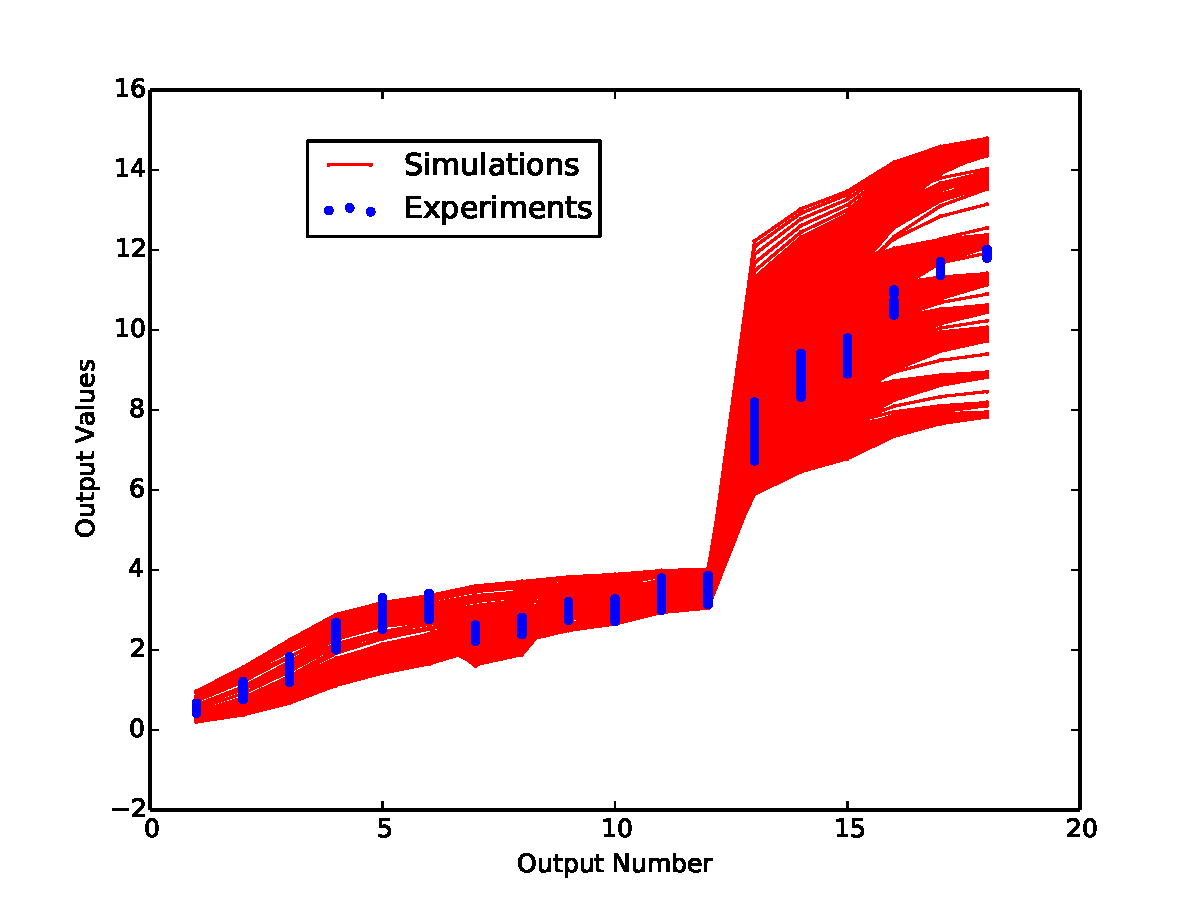
\includegraphics{figures/uqSanity.pdf}
\caption{Sanity check plot showing the parameter sweep data (red lines) against the experimental outputs (blue dots) for an MPI ping-pong benchmark}
\label{fig:uqSanityCheck}
\end{figure}

\section{Advanced Usage: Running Surrogate Construction and Sensitivity Analysis By Yourself}
Running the UQ analysis is involved. Help is available by contacting us at \url{sst-macro-help@sandia.gov}.
Documentation pending...


%\section{Applications/Capabilities}
%\label{sec:uqapp}
%
%\subsection{Forward UQ: uncertainty propagation and global sensitivity analysis}
%\label{subsec:fuq}
%
%The main technique we employ for forward UQ is the spectral Polynomial Chaos expansions (PCEs). 
%A PCE for a given model allows for a) efficient uncertainty propagation, b) very fast global sensitivity analysis, and 
%c) cheap surrogate model construction that can replace the original model in sampling-intensive studies such as calibration, 
%optimization, or, generally, inverse UQ.
%
%\subsubsection{Generic workflow:}
%
%A set of scripts that illustrate the essential forward UQ tasks is located in  \texttt{examples\_cpp/uq\_surr}.
%To enable running all scripts one should set an environment variable \texttt{UQTK\_SRC} that points to the location of UQTk.
%
%\begin{ShellCmd}
%setenv UQTK_SRC location/of/uqtk/in/your/computer
%\end{ShellCmd}
%
%
%A generic workflow consists of 4 steps:
%\begin{enumerate}
%\item Generate parameter samples to run the forward model at, for PC construction and validation, \texttt{gen\_sam.x}
%\begin{ShellCmd}
%gen_sam.x <domain_file> <sampling_type(Q/U)> <N_samples> <N_val>
%\end{ShellCmd}
%The list of arguments:
%\subitem \emph{domain\_file}: A file with \bgmth d \endmth rows and 2 columns. \bgmth d \endmth is the total number of parameters being explored.
%           The two columns are the lower and upper bound of the corresponding parameter.
%\subitem \emph{sampling\_type}: Q (Quadrature) or U (uniformly random). Note that currently in this script set, only Q is supported for further PCE generation.
%\subitem \emph{N\_samples}: Number of samples used for training, i.e. for building PCE.
%\subitem \emph{N\_val}:  Number of random samples generated for PCE validation. This can be set to 0 to skip validation.
%
%\item Run the black-box model, \texttt{model.x}
%\begin{ShellCmd}
%model.x
%\end{ShellCmd}
%This is a black-box model that takes no arguments. However, it expects two input files mparam.dat and minput.dat, and returns the function evaluations in the output file moutput.dat.
%\subitem \emph{mparam.dat}: a single column $d\times$1 of the parameters of interest, where d is the number of parameters 
%\subitem \emph{minput.dat}: controllable input in a matrix form, $N$$\times$$k$, where $k$ is the number of controllable parameters and $N$ is the number of values or model observables.
%\subitem \emph{moutput.dat}: the model output in a column format $N$$\times$1.
%
%This is the file that needs to be modified/provided by the user according to the model under study. Currently, a simple function $y=Ae^{Bx}+2Bx$ is implemented, where $A$ and $B$ are the parameters (mparam.dat) and $x$ is the single controllable input parameter (minput.dat). A user-created \texttt{model.x} should accept input files minput.dat and mparam.dat as described above, and it should produce an output file moutput.dat with the formats described above, 
%
%\item Obtain PCE for the model, \texttt{uq\_surr.x}
%\begin{ShellCmd}
%uq_surr.x <domain_file> <sampling_type(Q/U)> <N_samples> <N_val> \
%		<P_order> <moutput_surr_filename> <moutput_val_filename>
%\end{ShellCmd}
%
%The first four arguments coincide with those from \texttt{gen\_sam.x}, the rest of the arguments are:
%\subitem \emph{P\_order}: the PCE surrogate order. Polynomial series is truncated according to the total order.
%\subitem \emph{moutput\_surr\_filename}: model output file resulting from running \texttt{model.x} on training samples.
%\subitem \emph{moutput\_val\_filename}: model output file resulting from running \texttt{model.x} on validation samples.
%
%\item Postprocess, e.g. global sensitivity analysis, \texttt{pp\_sens.x} 
%\begin{ShellCmd}
%pp_sens.x
%\end{ShellCmd}
%
%The current implementation of the post processing script \texttt{pp\_sens.x} takes no arguments. It expects the presence of a PCE information file pccf\_all.dat, which is one of the outcomes of \texttt{uq\_surr.x}. The final global sensitivity results are saved in the \inlineshell{allsens.dat} file of dimensions $N$$\times$$d$, where each row corresponds to a single value for the controllable input (number of controllable inputs = N), and each column corresponds to the sensitivity index of a parameter (number of parameters = d).\\
%
%\medskip
%
%Note that one can run the model \texttt{model.x} in an \emph{online} regime by using the keyword "M" instead of filenames in
%\begin{ShellCmd}
%uq_surr.x <domain_file> <sampling_type(Q/U)> <N_samples> <N_val> <P_order> M M
%\end{ShellCmd}
%that effectively incorporates the steps 1-3 above.
%
%\subsubsection{Simple Example:}
%
%The script \texttt{example.x} incorporates the full workflow above for a test function $y=Ae^{Bx}+2Bx$. Try
%\begin{ShellCmd}
%example.x online
%\end{ShellCmd}
%which produces, in a newly created folder \texttt{test}, the sensitivity file \inlineshell{allsens.dat} with sensitivity indices with respect to $A$ and $B$ for all values of controllable input $x$.
%
%
%
%\end{enumerate}
%
%
%\subsubsection{How Forward UQ applies to \sstmacro}
%
%In the workflow described above, \sstmacro would replace the black-box simple model given by the equation, and \sstmacro parameters of interest would replace $A$ and $B$.   Note that while
%we could explore the entire \sstmacro parameter space using this workflow, the higher the dimensionality of the space the more time process takes, so we would also want to narrow it down to the most important parameters, usually by reasoning, inspection, or simple experimentation.  
%Also note that running an \sstmacro simulation can be considerably more expensive than evaluating an
%analytical model, which is why we typically construct a \textit{surrogate}, or an arbitrarily-complex polynomial that can approximate performance given by \sstmacro. 
%
%While the above workflow must currently be manually applied to \sstmacro data, we are working on automating this process and coming up with tutorials explaining how it is done.
%
%\subsection{Inverse UQ: parameter calibration and model validation}
%\label{subsec:iuq}
%
%UQTk relies on Bayesian inference methods for model parameter calibration. Model validation is a direct result of calibration 
%postprocessing. Indeed, a model is considered validated if the calibrated model parameters and the associated uncertainties can explain/predict available data well. 
%The library \texttt{uqtkmcmc} allows implementation of Bayesian calibration using Markov chain Monte Carlo (MCMC) methods. The MCMC technique essentially 
%searches the parameter space and compares model results with available data. Note that each parameter sample invokes a model evaluation, and often MCMC requires 
%many samples for properly estimating the uncertainties. In such cases, the full model, as a black-box, will be replaced by its surrogate, again as a black-box model, that is constructed by the forward UQ techniques described in Subsection~\ref{subsec:fuq}.
